\chapter{Проектирование и реализация математической модели средствами пакета MatLab Simulink}

В данной работе была проведена реализация модели физического перевернутого маятника с нелинейным регулятором. Графики поведения  фазового портрета формировались в графической среде Simulink в пакете прикладный программ MatLab, которая была выбрана из-за его достоинств:
\begin{enumerate}
\item[—] ввод блок при помощи палитры;
\item[—] вывод результата моделирования в реальном времени;
\item[—] возможность использования декомпозиций.
\end{enumerate}

\section{Перевернутый маятник и нелинейного регулятора }

Перевернутый маятник -- это модельный объект обычного физического маятника, у которого центр масс расположен выше точки опоры. Его можно стабильно подвешивать в этом перевернутом положении с помощью системы управления, которая контролирует угол наклона шеста и перемещает точку поворота горизонтально обратно под центр масс, когда он начинает падать, сохраняя равновесие. Пример такого маятника изображён на рисунке \ref{fig:10}.

\begin{figure}[h!]
\begin{center}
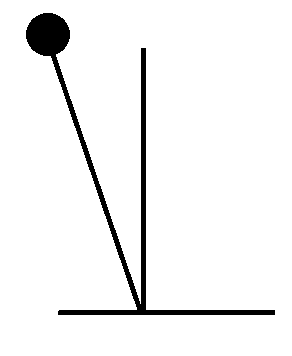
\includegraphics[angle=0,width=6cm]{fig/02.png}\\[2mm]
\caption{Модель перевернутого маятника}\label{fig:10}
\end{center}
\end{figure}


Цель системы перевернутого маятника заключается в том, чтобы управлять движением шара, чтобы он оставался в верхнем положении в течение как можно более длительного времени. Эта система является примером систем с перемееной стуктурой, так как ее структура может меняться в зависимости от текущего состояния системы.

Для управления движением перевернутого маятника используются нелинейные регуляторы, которые позволяют более эффективно управлять системой. Один из примеров нелинейного регулятора для управления перевернутым маятником -- это регулятор с обратной связью по состоянию, который использует линейную комбинацию состояний системы и нелинейную функцию для вычисления управляющего действия. Другой пример -- это регулятор с обратной связью по выходу, который использует выходной сигнал системы и нелинейную функцию для вычисления управляющего действия. Таким образом, нелинейные регуляторы позволяют более точно управлять перевернутым маятником, а также другими нелинейными системами, что делает их очень полезными в таких областях, как автоматическое управление, робототехника, электроника и другие, где требуется высокая точность и надежность управления.

Рассмотрим синтез закона управления, обеспечивающего существование скользящего режима для существенно нелинейного объекта, описываемого системой дифференциальное уравнение вида:

\begin{equation}\label{eq1}
    \begin{cases}
        \dot{x_1} = x_2\\
        \dot{x_2} = sin{x_1} + x_3\\
        \dot{x_3} = U(x_1, x_2, x_3),
    \end{cases}
\end{equation}
\noindent гиперповерхность $S(x_1,x_2,x_3)$ выберем следующего вида:
\begin{equation}\label{eq2}
    S(x_1,x_2,x_3) = c_1x_1+c_2x_2+c_3x_3,
\end{equation}
\noindent где коэффициент $c_3$ для простоты примем равным единице, а коэффициенты $c_1$ и $с_2$ выберем из условия симметрирования в пространстве гиперплоскости скольжения: 
\begin{equation}\label{eq2}
    c_1=c_2=c,
\end{equation}
\begin{equation}\label{eq2}
    c>0 . 
\end{equation}

\noindent В этом случае будет удовлетворяться условие устойчивости решения соответствующего дифференциального уравнения.
Уравнение гиперплоскости скольжения в этом случае запишется следующим образом:
\begin{equation}\label{eq2}
    S(x_1,x_2,x_3) = cx_1+cx_2+cx_3.
\end{equation}

Полная производная по времени $dS(x1,x2,x3)/dt$ взятая в силу системы \ref{eq1}, будет иметь вид:

\begin{equation}\label{eq6}
    \frac{dS}{dt} = cx_2 + c sin{x_1} + cx_3 + U(x_1, x_2, x_3)
\end{equation}
Подставим полученное выражение \ref{eq6} для производной в \ref{eq7}, 
\begin{equation}\label{eq7}
    S = -k([x_1]+[x_2]+...+[x_n])singS
\end{equation}


\noindent откуда найдем выражение для закона управления:

\begin{equation}\label{eq8}
     U= -k([x_1]+[x_2]+[x_3])singS-cx_2-csin{x_1}-cx_3.
\end{equation}

Полученный алгоритм управления содержит в себе операции взятия модуля и присвоения знака, которые легко реализуются с помощью цифровой системы управления. Кроме этого следует отметить, что нелинейности объекта управления входят в функцию управления непосредственно, то есть от нас не требуется обращать или дифференцировать нелинейности, входящие в структуру объекта. Это является существенным преимуществом предложенного метода перед другими методами синтеза нелинейных САУ.

\section{Построение математической модели перевернутого маятника с управляющим блоком}

Для построения математической модели маятника будем использовать MatLab и его расширение Simulink. Функциональная схема состоит из объекта управления, представляющего собой перевернутый маятник и нелинейного регулятора, формирующего требуемый разрывной закон управления \ref{eq8}. Из этого уравнения, мы видим, что это диффиринциальное уравнение второго порядка, поэтому чтобы его решить надо его проигтрегрировать 2 раза, в этом нам помогут интеграторы.

Регулятор состоит из линейной части (включающей в себя обратные связи по фазовым координатам $x_2,x_3$, показанный на рисунке \ref{fig:11}) и нелинейной части (включающей нелинейные блоки $sin()$ и модуль показанный на рисунке \ref{fig:04}).
\begin{figure}[h!]
\begin{center}
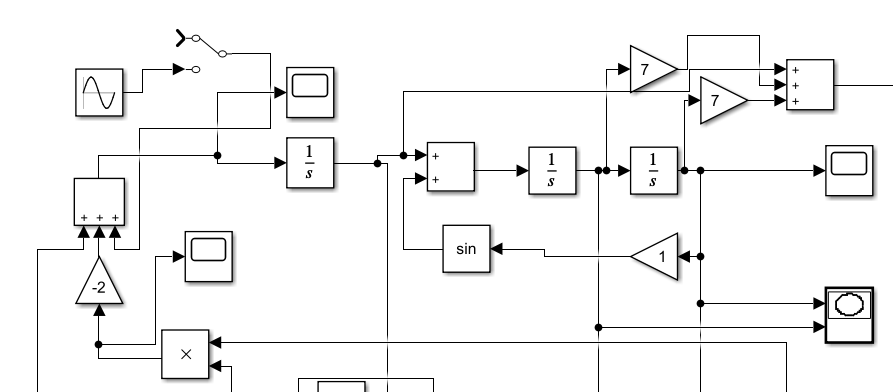
\includegraphics[angle=0,width=17cm]{fig/03.png}\\[2mm]
\caption{Фазовые координаты}\label{fig:11}
\end{center}
\end{figure}
\begin{figure}[h!]
\begin{center}
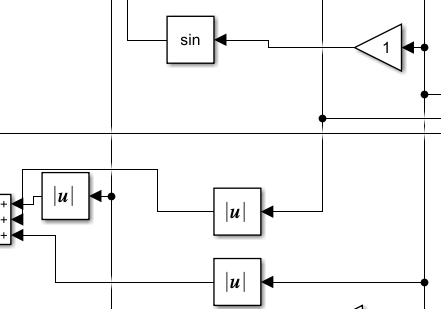
\includegraphics[angle=0,width=17cm]{fig/04.png}\\[2mm]
\caption{Нелинейный блок регулятора}\label{fig:04}
\end{center}
\end{figure}

Модель системы, сгенерированная в пакете прикладных программ Matlab, представлена на рисунке \ref{fig:02}. Для просмотра результатов используем блоки построение графика. Один для анализа поведения маятника, а второй для фазового портрета.


\begin{figure}[h!]
\begin{center}
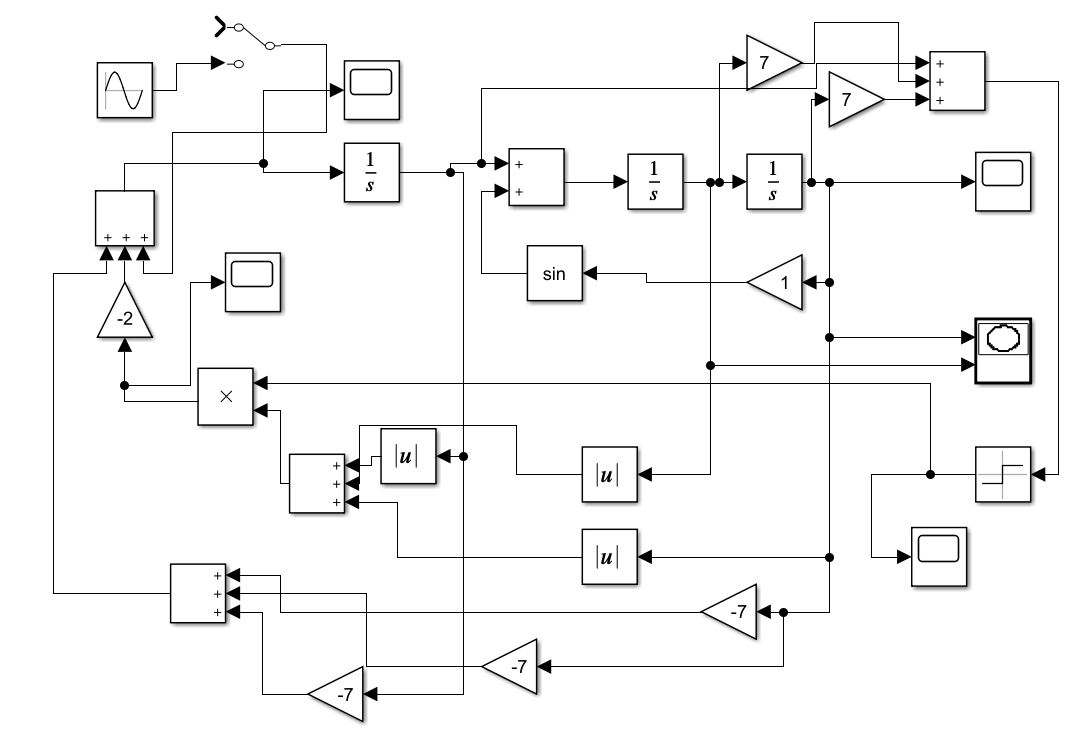
\includegraphics[angle=0,width=17cm]{fig/01.png}\\[2mm]
\caption{Структурная модель перевернутого маятника и нелинейнным регулятором}\label{fig:02}
\end{center}
\end{figure}

\section{Анализ результатов и подведение итогов в проведенной работы}

Разработанная программа предназначена для  создания математической модели с системой с переменной структурой в виде перевернутого маятника и нелинейного регулятора в среде визуального программирования. Чтобы проанализировать работу данной программы, выведем все имеющиемся графики.

Поведение системы в фазовом пространстве изображено на рисунке \ref{fig:05} Система попадает в скользящий режим, о чём свидетельствуют фазовые траектории, которые стягиваются в точке 0.

 \begin{figure}[h!]
\begin{center}
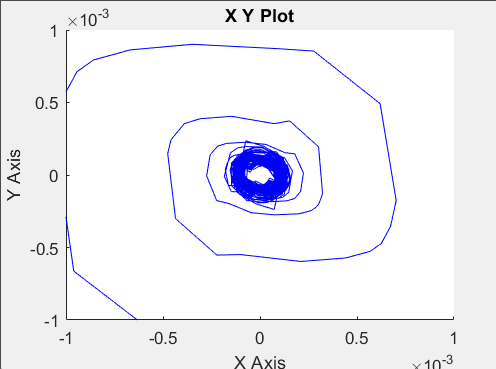
\includegraphics[angle=0,width=10cm]{fig/05.png}\\[2mm]
\caption{Фазовый портрет перевернутого маятника с нелинейнным регулятором}\label{fig:05}
\end{center}
\end{figure}

Что касается управляющего воздействия $U(x_1,x_2,x_3)$, поведение которого мы можем наблюдать на рисунке \ref{fig:06}, как и координаты ошибки управления - а рисунок \ref{fig:07} подтверждает тот факт, что система с переменной структурой попадает в скользящий режим, то есть изображающая точка колеблется с бесконечно большой частотой в некоторой малой окрестности гиперповерхности разрыва. 

\begin{figure}[h!]
\begin{center}
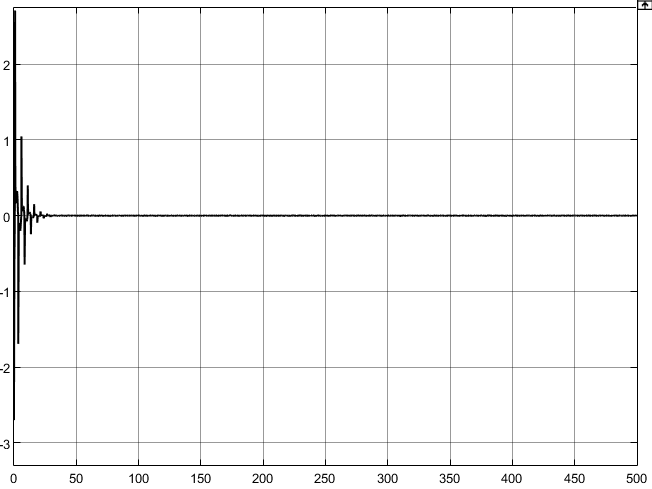
\includegraphics[angle=0,width=9cm]{fig/06.png}\\[2mm]
\caption{Управляющее воздействие перевернутого маятника с нелинейнным регулятором}\label{fig:06}
\end{center}
\end{figure}
Условия срабатывания переключений в системе показаны на рисунке \ref{fig:08}.
\begin{figure}[h!]
\begin{center}
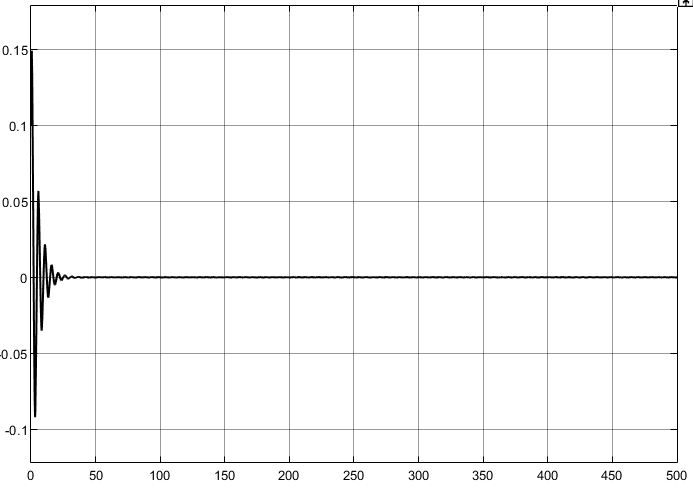
\includegraphics[angle=0,width=10cm]{fig/07.png}\\[2mm]
\caption{Координата ошибки перевернутого маятника с нелинейнным регулятором}\label{fig:07}
\end{center}
\end{figure}

\begin{figure}[h!]
\begin{center}
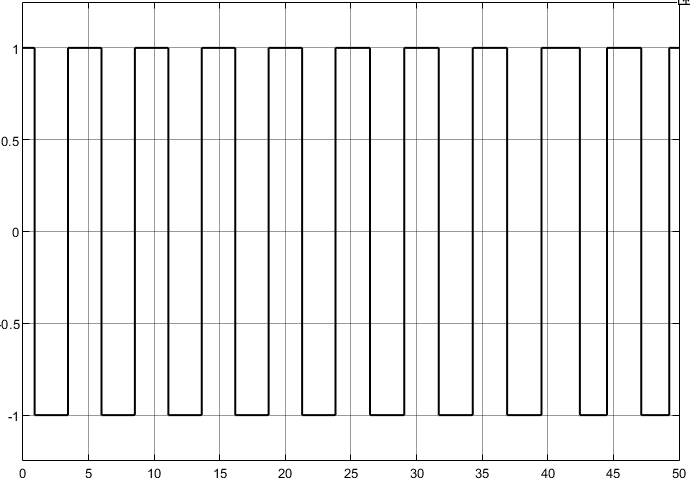
\includegraphics[angle=0,width=10cm]{fig/08.png}\\[2mm]
\caption{Переключения в системе с переменной структурой перевернутого маятника с нелинейнным регулятором}\label{fig:08}
\end{center}
\end{figure}

В результате анализа смоделированной системы с переменной структурой можно прийти к выводу о том, что система данного типа обладает свойством грубости, то есть нечувствительности к изменению параметров системы и инвариантности к внешним возмущениям.

Таким образом, системы с переменной структурой -- класс нелинейных систем с разрывным управлением. 
Системы в которых связи между функциональными элементами меняются тем или иным образом, в отличие от систем с фиксированной структурой, в которых совокупность функциональных элементов и характер связей между ними остаются неизменными.
